%--------------------------------------------------------------------------
% Dokumentenklasse
%--------------------------------------------------------------------------

% disable Warning for remreset Package
\RequirePackage{silence}
\WarningFilter{remreset}{The remreset package}

\documentclass[
	pagesize,
	fontsize=12pt,
	paper=a4,
	oneside,
   reqno
]{scrartcl}

%--------------------------------------------------------------------------
% Standartpackete 
%--------------------------------------------------------------------------
\usepackage[ngerman]{babel}               % Deutsch Silbentrennung
\usepackage[T1]{fontenc}                  % Font Type
\usepackage[utf8]{inputenc}               % Font Encoding
\usepackage{lmodern}                      % Latin Modern Font
\usepackage{csquotes}                     % Setzen von Zitaten
\usepackage{xspace}                       % setzten von Leerzeichen nach Abkürzungen
\usepackage{microtype}                    % für glättere Seitenränder
\renewcommand*\familydefault{\sfdefault}  % Serifenlose Schrift
%\renewcommand*\familydefault{\ttdefault} % Schreibmaschinenschrift

%--------------------------------------------------------------------------
% Extra Packages
%--------------------------------------------------------------------------

% Abkürzungspaket
\usepackage{acronym}

% Mathe Pakete
\usepackage{amsmath}
\usepackage{thmtools}
\usepackage{amsfonts}
\usepackage{amssymb}
\usepackage{mathtools}
\usepackage{gensymb}

% Listenumgebungen
\usepackage{listings}
\usepackage{paralist}
\usepackage{enumitem}
\usepackage{adjustbox}

% Demo Text
\usepackage{blindtext}

% Farb-Pakete
\usepackage{xcolor}
\usepackage{fancyvrb}
\usepackage{colortbl}

% Farbedefinitionen
\definecolor{htw}{RGB}{120, 184, 2}
\definecolor{ccW}{RGB}{255,255,255}
\definecolor{ccR}{RGB}{197,14,31}
\definecolor{ccG}{RGB}{113,113,113}
\definecolor{ccL}{RGB}{220,220,220}
\definecolor{ccS}{RGB}{0,0,0}
\definecolor{ccB}{RGB}{68,73,159}
\definecolor{ccD}{RGB}{0,0,80}

% Für erweiterte Tabellen
\usepackage{longtable}
\usepackage{tabularx}
\usepackage{float}
\usepackage{multirow}
\usepackage{makecell}
% \setlength{\tabcolsep}{0.5em}       % for the horizontal padding
% {\renewcommand{\arraystretch}{1.8}  % for the vertical padding
% \usepackage{ragged2e}
% \newcolumntype{R}[1]{>{\RaggedRight}p{#1}}

% Einheitenpaket
\usepackage[exponent-product = \cdot]{siunitx}
\sisetup{locale=DE}

\makeatletter
\renewcommand\@dotsep{5}
\makeatother

% Pakete für Grafiken
\usepackage{graphicx}
\usepackage{wrapfig}
\usepackage{overpic}
\usepackage{epstopdf}
\usepackage{caption}
\usepackage{subcaption}
% \captionsetup[subfigure]{list=true, font=normalsize, labelformat=brace, position=top} %setup für subfigure captions

% Diagramm-/Grafikerstellung
\usepackage{pstricks}
\usepackage{tikz}
\usetikzlibrary{math}
\usepackage{pgfplots}
\pgfplotsset{compat=1.5}
\usetikzlibrary{intersections,positioning,arrows,automata,calc,patterns,shapes.multipart,fit,backgrounds,decorations.pathreplacing}
\usetikzlibrary{decorations,shapes.geometric}
\usetikzlibrary{matrix,calc,angles,positioning,quotes}
% \usepackage{tikz-uml}

\usepackage{pgfkeys}
\usepackage{pgfopts}
\usepackage{ifthen}
\usepackage{xstring}
\usepackage{calc}
\usepackage{pst-plot,pst-bar,pst-node} % Balkendiagramme
\usepackage{capt-of}
\usepackage{incgraph} % Fullscreen Images
\usepackage{pdfpages} % Include external pdf pages

\usepackage{latexsym}
\usepackage{censor}
\usepackage{here}
% \StopCensoring        % Auskommentiert wird der Text entschwaerzt 
% \censor{Oszilloskop}  % Befehl zum einschwärzen
\usepackage{trfsigns}   % Transformation Symbol o---o \laplace and \Laplace
\usepackage{circuitikz}

\usepackage{multido}

% Verlinkungen im Text
\usepackage{url}
\usepackage{hyperref}
\PassOptionsToPackage{hyphens}{url}
\hypersetup{hidelinks}
\urlstyle{same}

%--------------------------------------------------------------------------
% Eigene Befehle
%--------------------------------------------------------------------------

% \renewcommand{\thesection}{\arabic{section}} % Section startet mit 1.0 und nicht mit 0.1

%------------sectioning command-------------------
% The sectioning command one level down the hierarchy from \subsubsection is called \paragraph followed by \subparagraph
% to include this in your table of contents

% for paragraph
\setcounter{tocdepth}{4}
\setcounter{secnumdepth}{4}
% for subparagraph
\setcounter{tocdepth}{5}
\setcounter{secnumdepth}{5}

%------------Zitate-------------------------------
\newcommand*{\zitat}[2]{%
   \normalfont\small
   \begin{quote}
   \glqq#1\grqq \par
   #2
   \end{quote}
   \normalsize
}
\newcommand*{\zitatmitueberschrift}[3]{%
   \normalfont\small
   \begin{quote} #3
   \glqq#1\grqq \par
   #2
   \end{quote}
   \normalsize
}
\newcommand*{\zitext}[2]{%
   \glqq#1\grqq\ %
   [#2]%
}

%-----------Seitendesign--------------------------
\usepackage[width=15.5cm, height=23cm, includeheadfoot]{geometry}
\geometry{paper=a4paper}
% \usepackage[left=6cm,right=1cm,top=1.5cm, bottom=1cm, includeheadfoot]{geometry}
% \newgeometry{oneside}
% \setlength{\voffset}{0cm}
\setlength{\headheight}{1.1\baselineskip} % increase headheight
\setlength{\footheight}{28.99998pt}       % increase foodheight
\setlength{\parindent}{0cm}               % Einrücken nach \newline
\setlength{\footskip}{86pt}               % Move Footer down
% \setlength{\topmargin}{0cm}
% \setlength{\marginparsep}{0.5cm}
% \setlength{\marginparwidth}{1.5cm}
% \setlength{\textwidth}{16cm}
% \setlength{\textheight}{23cm}
% \setlength{\oddsidemargin}{1cm}
% \setlength{\evensidemargin}{2cm}

%----------Kopf & Fußzeile------------------------
% \usepackage[headsepline,footsepline]{scrpage2}
\usepackage[headsepline]{scrlayer-scrpage}
\pagestyle{scrheadings}
\clearpairofpagestyles
\ihead{\headmark}
\automark{section}
\chead{}
\ohead{
\includegraphics[scale=0.09]{Bilder/HTWLogoKopfzeile.png} \nocite{HTWklein}}
\ifoot{Aaron Zielstorff\\ 567183}
\cfoot{\pagemark}
\ofoot{M1 Angewandte Mathematik}

%--------------------------------------------------------------------------
% Beginn des Dokuments
%--------------------------------------------------------------------------
\begin{document}

%----------Deckblatt----------------------------- 
\begin{titlepage}
   \pagestyle{empty} % setzt Pagestyle-Befehl

   % HTW Logo
   \begin{flushright}
   
\includegraphics[scale=.07]{Bilder/LogoHTWBerlin.png}  \nocite{HTWgross}
   \end{flushright}

   \vspace{1cm}

   % Titel
   \begin{center}
      \Huge{\textbf{Projekt Zeitaufgelöste Photolumineszenz: 
      Angewandte Mathematik (M1)}} \\
   \end{center}

   \vspace{3cm}

   % Name
   \begin{flushleft}
      \begin{tabular}{l l}
         \textbf{Name:}    & Aaron Zielstorff   \\
         \textbf{Mtr.Nr.:} & 567183             \\
      \end{tabular}
   \end{flushleft}

   \vspace{1cm}

   % Daten
   \begin{tabular}{l l}
      \textbf{Fachbereich:}   & FB1                                              \\
      \textbf{Studiengang:}   & M.\xspace Elektrotechnik                         \\
      \textbf{Fachsemester:}  & 1.\xspace FS                                     \\
      \textbf{Fach:}          & M1 Angewandte Mathematik                         \\
      \textbf{Dozent:}        & Prof.\xspace Dr.\xspace A.\xspace Zeiser         \\
      \textbf{Abgabe am:}     & 20.\xspace März 2022                             \\ 
   \end{tabular}
\end{titlepage}
\clearpage

%--------Inhaltsverzeichnis-----------------------
\renewcommand{\contentsname}{Inhaltsverzeichnis}
\tableofcontents
\clearpage

%--------Abbildungsverzeichnis--------------------
\renewcommand{\listfigurename}{Abbildungsverzeichnis}
\renewcommand*{\figurename}{Abb.}
\listoffigures
% \clearpage

%--------Tabellenverzeichnis----------------------
\renewcommand*{\listtablename}{Tabellenverzeichnis}
\renewcommand*{\tablename}{Tab.}
\listoftables
\clearpage


%---------Kapitel/Text----------------------------

\section{Einleitung}

Perowskit-Solarzellen sind der neue Stern am Himmel der Photovoltaik. Innerhalb von wenigen Jahren sind diese neuartigen Materialien zu konkurrenzfähigen Dünnschicht-Solarzellen mit weit über 20\% Wirkungsgrad erwachsen. Daraus begründen sich die enorme Popularität und auch die vielen Hoffnungen an diese Halbleiter-Materialklasse. Dennoch gibt es noch zahlreiche Probleme und ungeklärte Fragestellungen, die die Forschung adressieren kann. Andreas Bartelt und seine Gruppe untersuchen an der HTW Berlin diese Materialien mithilfe von zeitaufgelösten Photolumineszenz-Spektren (TRPL, \textit{time resolved photo-
luminescence}): das Material wird mithilfe eines Lasers angeregt und die aus der Anregung entstehende Aussendung von Licht in Abhängigkeit von der Zeit gemessen. \\
Um aus den experimentellen Daten Rückschlüsse auf Lebensdauern und Hinweise auf effizienzlimitierende Prozesse in den neuen Materialien zu ziehen, ist eine Simulation der Dynamiken im Halbleiter notwendig. In dieser Hausarbeit sollen Sie die Grundlagen einer solchen Simulation entwickeln. \\
Der Halbleiter der Dicke $d$ zwischen zwei Materialien wird gleichmäßig in der Fläche bestrahlt und erzeugt so eine Ladungsträgerdichte $u$ im Halbleiter (siehe \autoref{fig:Bild1}). Die Abhängigkeit von $u$ in der Ebene senkrecht zur Dicke kann in guter Näherung vernachlässigt werden, so dass die Ladungsträgerdichte eine
Funktion der Zeit $t$ und der Tiefe $z$ ist. Die Elektronendynamik im Halbleiter nach der Bestrahlung wird durch eine Diffusionsgleichung modelliert [3]. Die Ladungsträgerdichte $u(t,z)$ im Halbleiter genügt der parabolischen Differenzialgleichung

\begin{align}
   \label{eq:eq1}
   \frac{\partial u}{\partial t} = D\frac{\partial^2 u}{\partial z^2} - (k_1 + k_2N_D)u - k_2u^2 + s(t, z), \quad t \geq t_0, 0 < z < d
\end{align}

mit der Anfangsbedingung

\begin{align}
   \label{eq:eq2}
   u(t_0, z) = 0, \quad 0 \geq z \geq d
\end{align}

und den Randbedingungen

\begin{align}
   \label{eq:eq3}
   D\frac{\partial u}{\partial z}(t, 0) = S_Lu(t, 0), \quad D\frac{\partial u}{\partial z}(t, d) = -S_Ru(t, d), \quad t \geq t_0
\end{align}

\begin{figure}[H]
   \centering
   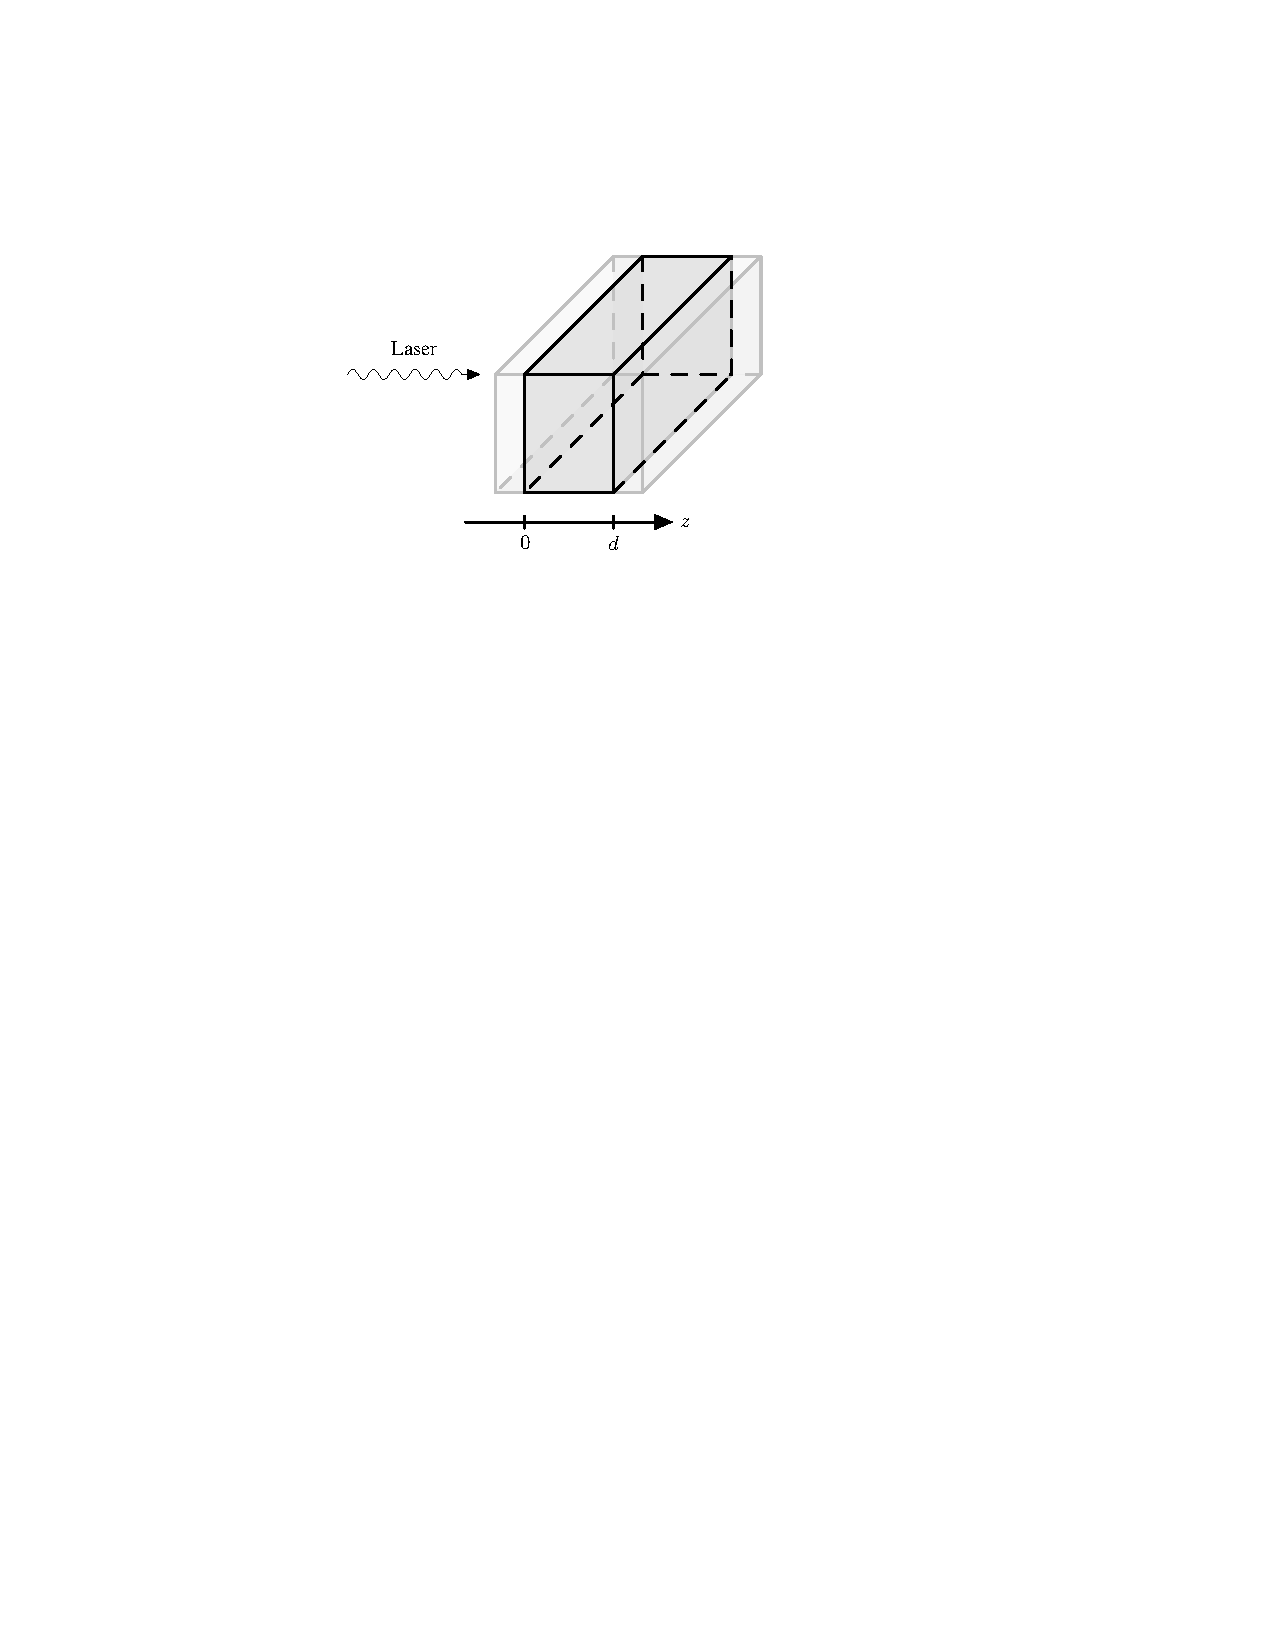
\includegraphics[scale=0.7]{Bilder/Bild1.pdf}
   \caption[Skizze des Aufbaus der Probe]{Skizze des Aufbaus der Probe. Der Halbleiter aus Peroskit liegt zwischen zwei Materialien und wird in der Ebene senkrecht zu $z$ als unendlich ausgedehnt angenommen. Die Bestrahlung mit Laserlicht erfolgt gleichmäßig aus der Richtung $z < 0$.}
   \label{fig:Bild1}
\end{figure}

Hier ist $s(t,z)$ die Ladungsträgerdichte, die durch die Bestrahlung pro Zeiteinheit erzeugt wird, $D$ die Diffusionskonstante, $N_D$ die Dotierungsdichte, $k_1$ bzw.\xspace $k_2$ die Rekombinationskonstanten (Shockley Read Hall Rekombination, bzw.\xspace direkte Rekombination) und $\alpha$ die Absorptionskonstante. Die Konstanten $S_L$ $(z = 0)$ bzw.\xspace $S_R$ $(z = d)$ bestimmen die Rekombinationsraten an den jeweiligen Grenzschichten. \\

In dieser Arbeit sollen folgende Parameter verwendet werden

\begin{table}[H]
   \centering
   \resizebox{0.7\textwidth}{!}{%
      \begin{tabular}{l|l|l|l|l|l|l|l|l}
         Parameter & $d$                  & $D$                               & $K_1$                       & $k_2$                             & $N_D$                             & $S_L$                       & $S_R$                       & $\alpha$                    \\ \hline
         Einheit   & $\left[\mu m\right]$ & $\left[\frac{{cm}^2}{s}\right]$   & $\left[\frac{1}{s}\right]$  & $\left[\frac{{cm}^3}{s}\right]$   & $\left[\frac{1}{{cm}^3}\right]$   & $\left[\frac{cm}{s}\right]$ & $\left[\frac{cm}{s}\right]$ & $\left[\frac{1}{cm}\right]$ \\ \hline
         Wert      & $0.3$                & $0.003$                           & $10^6$                      & $10^{-8}$                         & $10^{15}$                         & $10$                        & $10^5$                      & $10^5$  
      \end{tabular}%
   }
   \caption{Verwendete Parameter}
   \label{tab:Tabelle1}
\end{table}

\textbf{Achtung:} Verwenden Sie in der Simulation durchgehend $\mu m$ und $\mu s$ als Einheit! \\

Die Simulation von \autoref{eq:eq1} wird schrittweise entwickelt. In \autoref{sec:FiniteDifferenzen} wird zunächst die Zeitabhängigkeit vernachlässigt und eine Diskretisierung im Raum der stationären Gleichung mittels finiter Differenzen entwickelt. Der folgende \autoref{sec:ImpliziteEinschrittverfahren} untersucht eine Klasse von numerischen Verfahren zur Lösung von Anfangswertproblemen, die besonders gut für den vorliegenden Fall geeignet sind. Im letzten \autoref{sec:ZeitaufgeloesteSimulation} werden beide Ansätze mithilfe der Linienmethode kombiniert und eine numerische Lösung der Ausgangsgleichung berechnet.

\clearpage

\section{Finite Differenzen der stationären Gleichung} \label{sec:FiniteDifferenzen}

In diesem Teil der Arbeit soll die stationäre Verteilung der Ladungsträger, d.\xspace h.\xspace für den Fall $\partial u/\partial t = 0$, bei kontinuierlicher Bestrahlung modelliert werden. In diesem Fall ist die Gleichung durch

\begin{align}
   \label{eq:eq4}
   D\frac{\partial^2 u}{\partial z^2} - (k_1 + k_2N_D)u - k_2u^2 = -s(z), \quad 0 < z < d
\end{align}

mit Randbedingungen

\begin{align}
   \label{eq:eq5}
   D\frac{\partial u}{\partial z}(0) = S_Lu(0), \quad D\frac{\partial u}{\partial z}(d) = -S_Ru(d)
\end{align}

gegeben. Hier ist $s(z)$ die Ladungsträgerdichte, die pro Zeiteinheit durch die externe Quelle erzeugt wird. \\

Die Gleichung soll näherungsweise mithilfe der Finite Differenzen Methode gelöst werden [4] (benötigte Abschnitte werden auf Moodle bereitgestellt). Dazu wird das Gebiet $z \in [0, d]$ in $M$ gleich große Intervalle der Länge $h$ aufgeteilt und die Knotenpunkte mit $0 = z_0 < z_1 < ... < z_N = d$ bezeichnet. Die genäherte Ladungsdichte an den Stellen $z_i$ wird mit $u_i$ bezeichnet, d.\xspace h.\xspace es soll

\begin{align*}
   u_i \approx u(z_i), \quad i = 0, 1, ..., N
\end{align*}

gelten. Für diese Werte wird ein Gleichungssystem hergeleitet und anschließend numerisch gelöst. Zwischenzeitlich werden Hilfsknoten an den Stellen $z_{-1} = -h$ und $z_{N+1} = d + h$ mit Werten $u_{-1}$ und $u_{N+1}$ verwendet, die jedoch später durch die Randbedingungen eliminiert werden.

\subsection{Lineare stationäre Gleichung}

Im ersten Schritt soll nur der in $u$ lineare Anteil der \autoref{eq:eq4} ohne den quadratischen Term $-k_2u^2$ untersucht werden:

\begin{align}
   \label{eq:eq6}
   D\frac{\partial^2 u}{\partial z^2} - ku = -s(z), \quad 0 < z < d
\end{align}

mit $k = k_1 + k_2N_D$. Die Randbedingungen sind weiterhin durch \autoref{eq:eq5} gegeben. \\

Die Behandlung der stationären Gleichung erfolgt ähnlich zu der in [4, Abschnitt 8.8] beschriebenen Methode. Jedoch werden die Randbedingungen unterschiedlich behandelt. Folgende Aufgaben wurden bearbeitet.

\subsubsection{Vorgehen aus [4, Abschnitt 8.8] angewendet auf \autoref{eq:eq6}}



\clearpage

\section{Implizite Einschrittverfahren} \label{sec:ImpliziteEinschrittverfahren}

\clearpage

\section{Zeitaufgelöste Simulation} \label{sec:ZeitaufgeloesteSimulation}

\clearpage

%---------Quellen---------------------------------
\newpage
\newcount\Quellennummer
\Quellennummer=1

\renewcommand\refname{Literaturverzeichnis}
\addcontentsline{toc}{section}{Literaturverzeichnis}

\begin{thebibliography}{999}
{\setlength{\emergencystretch}{3cm}%

\bibitem[\the\Quellennummer]{HTWgross}
HTW-Logo auf dem Deckblatt\par
\url{https://de.wikipedia.org/wiki/Datei:Logo_HTW_Berlin.svg} \par
 Stand: 17.08.2018 um 14:49 Uhr

\advance\Quellennummer by 1
 
\bibitem[\the\Quellennummer]{HTWklein}
HTW-Logo in der Kopfzeile\par
\url{http://tonkollektiv-htw.de/} \par
 Stand: 17.08.2018 um 14:53 Uhr

\advance\Quellennummer by 1

\bibitem[\the\Quellennummer]{PervoskitSolarCells}
Baloch, Ahmer A. B. \textit{et al:} \glqq Analysis of Photocarrier Dynamics at Interfaces in Pervoskite Solar Cells by Time-Resolved Photoluminescensce\grqq{}, The Journal of Physical Chemistry C, Seiten 26805 - 26815 (2018).

\advance\Quellennummer by 1

\bibitem[\the\Quellennummer]{NumericalAnalysis}
Atkinson, Kendall E. und Han, Weimin: \glqq Elementary Numerical Analysis\grqq{}, J. Wiley \& Sons, Hoboken, NJ (2004).

\advance\Quellennummer by 1

}
\end{thebibliography}

\end{document}